\section{Numerical Methods}\label{app:numerical}

%==============================================================================
\subsection{GRMHD Consistency and Convergence}\label{app:resolution_study}

\note{Hector to provide first draft.}

\op{I can put this in}
\note{Brief general discussion of Porth et al. and Olivares et al.}

\note{Comparison of GRMHD output from Illinois/Frankfurt/HAMR}

\note{Comparison of GRMHD output from Illinois at multiple resolutions}

%==============================================================================
\subsection{Radiative Transfer Consistency and Convergence}
\label{app:radtrans}

\note{Ben to provide first draft.}

Two studies have been undertaken within the EHT comparing radiative transfer methods used to evaluate models.  The first, \cite{2020ApJ...897..148G}, 

Brief discussion of Gold et al., Prather et al.

\begin{figure}
  \centering
  %\note{altex}
  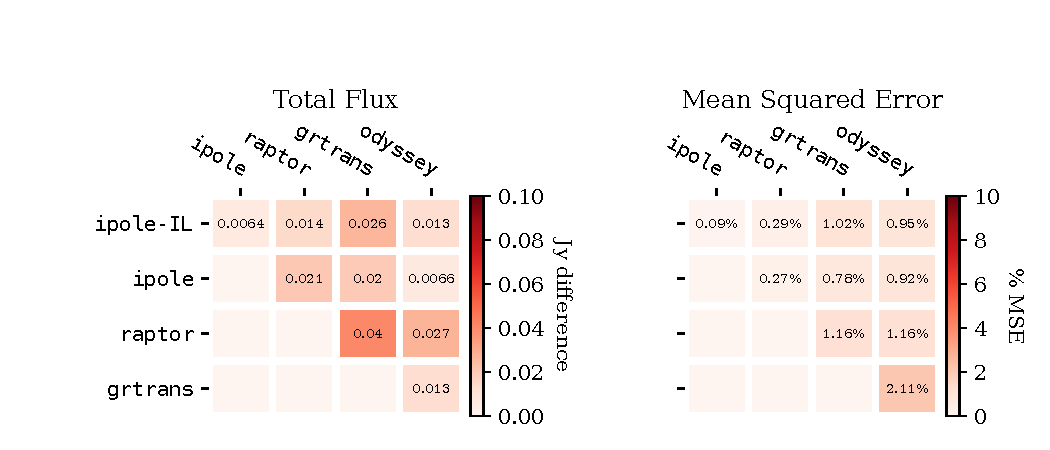
\includegraphics{figures/grmhd_hi_IntegratedUnpolarizeds_plot.pdf}
  \caption{}
  \label{fig:radtrans_grmhd_comp}
\end{figure}

Field of View

Resolution

%==============================================================================
\subsection{Spectral Energy Distribution Consistency and Convergence}

\ckc{CK will do first pass}

\begin{figure*}
    \centering
    %\includegraphics{}
    \note{altex: plot GRRT flux vs SED flux at different wavelengths.  Demonstrates that we have good agreements for 230GHz.  Demonstrate that NIR may require Monty Carlo calculations due to inverse Compton.  Demonstrate some 86GHz images require larger FoV but they are ruled out anyway and would not affect the results.}
    \caption{Comparing GRRT flux from Monte Carlo calculations.  The three columns are 86GHz, 230GHz, and NIR, respectively.  GRRT is only used to spot check x-ray and does not have a corresponding scatter plot.}
    \label{fig:sed_vv}
\end{figure*}

%==============================================================================
\subsection{Cross-Validations}

\ckc{Christian to provide figure}

\begin{figure*}
    \centering
    %\includegraphics{}
    \note{altex: scatter plot between, e.g., Illinois and Frankfurt models for the different measurable.}
    \caption{Comparing model predictions from different modeling pipelines.  ...}
    \label{fig:xv}
\end{figure*}
